% В этом шаблоне используется класс spbau-diploma. Его можно найти и, если требуется, 
% поправить в файле spbau-diploma.cls
\documentclass{spbau-diploma}
\begin{document}
% Год, город, название университета и факультета предопределены,
% но можно и поменять.
% Если англоязычная титульная страница не нужна, то ее можно просто удалить.
\filltitle{ru}{
    chair              = {Кафедра математических и информационных технологий},
    title              = {Решение задачи восстановления клональных деревьев репертуара антител с помощью данных парного иммуносеквенирования},
    % Здесь указывается тип работы. Возможные значения:
    %   coursework - Курсовая работа
    %   diploma - Диплом специалиста
    %   master - Диплом магистра
    %   bachelor - Диплом бакалавра
    type               = {master},
    position           = {студента},
    group              = 605,
    author             = {Черниговская Мария Александровна},
    supervisorPosition = {к.\,ф.-м.\,н., постдок \\Калифорнийского университета в Сан-Диего\\},
    supervisor         = {Сафонова Я.\,Ю.},
    reviewerPosition   = {??\\},
    reviewer           = {Шугай М.\,А.},
    chairHeadPosition  = {д.\,ф.-м.\,н., профессор},
    chairHead          = {Омельченко А.\,В.},
    % university = {САНКТ-ПЕТЕРБУРГСКИЙ АКАДЕМИЧЕСКИЙ УНИВЕРСИТЕТ},
    % faculty = {Центр высшего образования},
    % city = {Санкт-Петербург},
    % year             = {2013}
}
\filltitle{en}{
    chair              = {Department of Mathematics and Information Technology},
    title              = {Clonal trees reconstraction of antobody repertoires using paired single cell sequencing data},
    author             = {Maria Chernigovskaya},
    supervisorPosition = {Ph.D., postdoc at UCSD\\},
    supervisor         = {Yana Safonova},
    reviewerPosition   = {???\\},
    reviewer           = {Mikhail Shugay},
    chairHeadPosition  = {professor},
    chairHead          = {Alexander Omelchenko},
}
\maketitle
\tableofcontents

\section*{Реферат}

В данной работе описывается алгоритм  pairedAntEvolo, который позволяет анализировать данные парного иммуносеквенирования, полученные методом секвенированмя одиночных клеток. Алгоритм предназначен для разбиения репертуара B-клеток на клональные линии и восстановления эволюционных деревьев внутри каждой линии.  \\

\textbf{Ключевые слова:} парное иммуносеквенирование, секвенирование одиночных клеток, клональные линии, клональные деревья, B-клетки, репертуар антител, созревание лимфоцитов, адаптивный иммунный ответ

% -------------------------------------------------------------------------------------------

\section{Введение}

% Какие-то вводные слова
Развитие иммунной системы обусловило возможность существования сложно организованных многоклеточных организмов. Она распознает множество разнообразных возбудителей, от вирусов до паразитических червей, и отличает их от биомолекул клеток. Конечной целью работы иммунной системы является ликвидация чужеродного агента, которым может оказаться болезнетворный микроорганизм, инородное тело, ядовитое вещество или переродившаяся клетка самого организма. Различают врожденную и адаптивную иммуную систему. Задача врожденной иммунной системы давать быстрый иммунный ответ на ограниченное число патогенов, но она может справиться не со всем. Например, есть бактерии, которые умеют быстро мутировать и заставляют иммунную систему быстро адаптироваться к происходящему. Для этого у организмов начиная с рыб появилась адаптивная имунная система, которая не только умеет обучаться и отвечать практически на что угодно, но и запоминает результат иммунного ответа. 

% Мы будем смотреть на В-клетки
Важнейшим элементом адаптивной иммунной системы являются В-клетки. В-клетки производят специальные белки ---  антитела, которые циркулируют в крови и в лимфе. Антитела распознают и связываются с поверхностными белками вирусов и бактерий --- антигенами, и участвуют в их нейтрализации.  

% Устройство антитела + VDJ-рекомбинация
Молекула антитела состоит их двух пар различных белков, которые называются тяжелая и легкая цепь.  Вариабельные части тяжелой и легкой цепи образуют сайт связывания с антигеном и определяют специфичность данного антитела, то есть определяют, с каким именно антигеном будет связываться конкретное антитело. Таким образом, для того, чтобы имунная система могла бороться с огромным количеством потенциальных антигенов, В-клетки должны уметь синтезировать большое количество различных антител. Так как количество возможных антигенов много больше числа генов, которые можно закодировать в ДНК, существуют специальные процессы, которые повышают разнообразие антител: VDJ-рекомбинация, спаривание тяжелой и легкой цепи, соматический гипермутагенез и клональная селекция. 


\begin{figure}[h!]
    \centering
    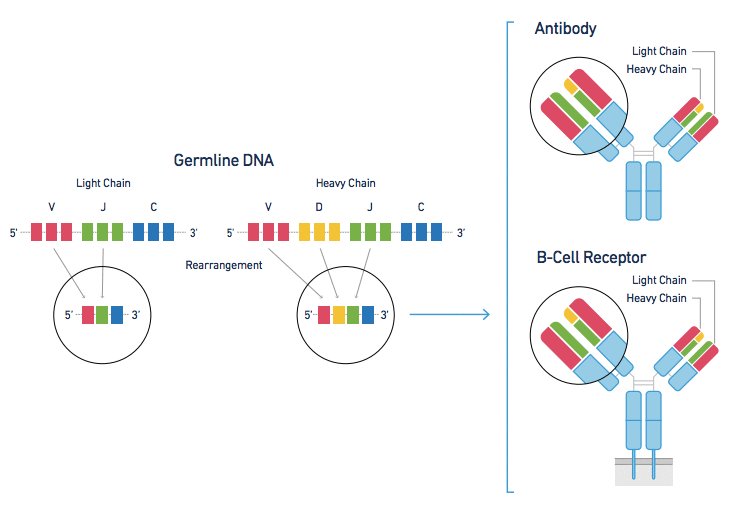
\includegraphics[width=.9\textwidth]{figures/10x_vdj_recombination.png}
    \caption{\textbf{ПЕРЕРИСОВАТЬ} Схематичное описание VDJ-рекомбинации. В геноме присутствуют три группы генов: V, D и J гены, которые похожи внутри каждой группы. После рекомбинации тяжелая цепь содержит в себе по одному конкретному гену V, D и J, легкая цепь --- только V и J. Сперва рекомбинирует тяжелая цепь: на первом этапе рекомбинации вырезается случайное количество D-сегментов с конца и случайное количество J-сегментов с начала. На втором этапе вырезается случайное количество конечных V-сегментов и все D-сегменты, кроме последнего. На стыках V-D и D-J происходят случайные мутации и вставки. Лишние V- и J-гены затем вырезаются в процессе транскрипции. В итоге, оставшиеся V-, D и J- гены вместе с константной частью образуют ген тяжелой цепи иммуноглобулина. Получившаяся в ходе рекомбинации тяжелая цепь тестируется на продуктивность. Если цепь не работает, то рекомбинирует вторая аллель. Если обе цепи не работают, то В-клетка погибает. Затем, аналогично тяжелой цепи, рекомбинирует легкая цепь. Если рекомбинация прошла успешно, то белки тяжелой и легкой цепь соединяются вместе и образуют антитело. 
сегменты. }
    \label{10x_vdj_recombination}
\end{figure}

% Откуда получаются деревья
VDJ-рекомбинация уникальным образом меняет геном гомопоэтической стволовой клетки и превращает ее в В-клетку. После того, как В-клетка успешно связалась с антигеном, она перемещается в герминальный центр и начинает делиться. В получившихся клетках-клонах специальный фермент вносит соматические гипермутации в вариабельную часть антигена, для того, чтобы улучшить связываемость антитела с антигеном. Клетки с нефункциональными рецепторами и клетки подозрительные на аутоиммунные отсеиваются, полезные клетки стимулируются к дальшейшему делению и мутациям. В результате такого эволюционного процесса образуются клональные семейства В-клеток. 

% Rep-seq vs single-cell
Для того, чтобы изучать имунную систему, существует несколько технологий секвенирования, которые позволяют восстанавливать вариабельную часть генов иммуноглобулина. Наиболее распространенное семейство технологий называется Rep-seq (Repertoire sequencing, ~\cite{pmid22043864}), которое позволяет с очень высокой точностью определить частоты антител встречающихся в образце. (Что-то написать про саму технологию(??). В общем, это обычное секвенирование кДНК с правильно подобранными праймерами, которые садятся на консервативный кусок в начало V-гена). Недостатком этих технологий является то, что в процессе секвенирования теряется важная информация о парности цепей, то есть какие именно тяжелые и легкие цепи образовывали вместе антитело. Не так давно появилась технология, которая позволяет секвенировать РНК антигенов с помощью одиночных клеток и сохраняет информацию о парности цепей. Для этого к РНК пришиваются молекулярные и клеточные баркоды. К сожалению, на текущий момент не существует общепринятого и стабильного протокола, но пока коммерческая компания 10х genomics являются лидерами по качеству парных данных.

% Цель работы
Целью данной работы является анализ реальных данных парного иммуносеквенирования и разработка метода восстановления клональных деревьев с помощью данных этого вида. 


% -------------------------------------------------------------------------------------------

\subsection{Мотивация}

% Репертуар имеет структуру! Это не просто множество, а дерево
В большинстве исследований (найти статью) репертуар рассматривается как множество антител, однако клональные деревья позволяют использовать дополнительную информацию о его структуре. При активном имунном ответе происходит активное деление полезных В-клеток, и скорее всего важные антитела будут содержаться в самых больших деревьях. Также построение клональных деревьев по данным временных серий позволяет изучать динамику имунного ответа (найти статью,~\cite{stern2014b} не совсем то). Для того, чтобы установить, в какой день наблюдался самый сильный иммунный ответ, можно следить за изменением размера самых больших деревьев. Также можно изучать, какие именно мутации оказались самыми полезными и привели к наибольшему распространению клона.     

% Зачем строить клональные деревья
А еще лучше смотреть на парный репертуар, чтобы не строить мифические деревья, потому что есть allelic inclusion. И мы не можем собрать антитело, пока не знаем обе цепи (и даже если знаем, то тоже сложно).


% -------------------------------------------------------------------------------------------

\subsection{Постановка задачи}

Биологическая и математическая

% Проанализировать данные

% Разработать алгоритм

% -------------------------------------------------------------------------------------------

\subsection{Существующие решения}

% Для одной цепи
Все умеют строить по одной цепи. 

% Для двух цепей (bracer)
По двум тоже умеют, но очень плохо.

% -------------------------------------------------------------------------------------------

\section{Анализ реальных данных}

% Описание технологии
На текущий момент компания 10x genomics~\cite{pmid28091601} является лидером по производству парных данных. Их технология секвенирования одиночных иммунных клеток (рис.~\ref{10x_pipeline}) позволяет с высокой точностью обработать от 100 до 10000 клеток в одном семпле. Для того, чтобы запомнить информацию о том, какие цепи экспрессирует конкретная клетка, используют клеточные и молекулярные баркоды (рис.~\ref{10x_barcodes}) . Клеточные баркоды позволяют отметить последовательности, которые относятся к одной клетке.  Молекулярные баркоды нужны для того, чтобы восстановить последовательности после амплификации. Помеченные двумя баркодами последовательности секвенируются с помощью парных ридов (150 нуклеотидов), которые затем собираются в контиги с помощью CellRanger VDJ. Затем происходит аннотация --- контиги выравниваются на базу известных V, D, J сегментов (гермлайн), и последовательности с плохим выравниванием отфильтровываются. Для оставшихся последовательностей определяется лучшее выравнивание на V и J сегменты. В конечном итоге получается набор последовательностей цепей иммуноглобулинов с клеточным баркодом и предполагаемыми V и J сегментами, из которые были выбраны в ходе VDJ-рекомбинации.

\begin{figure}[h!]
    \centering
    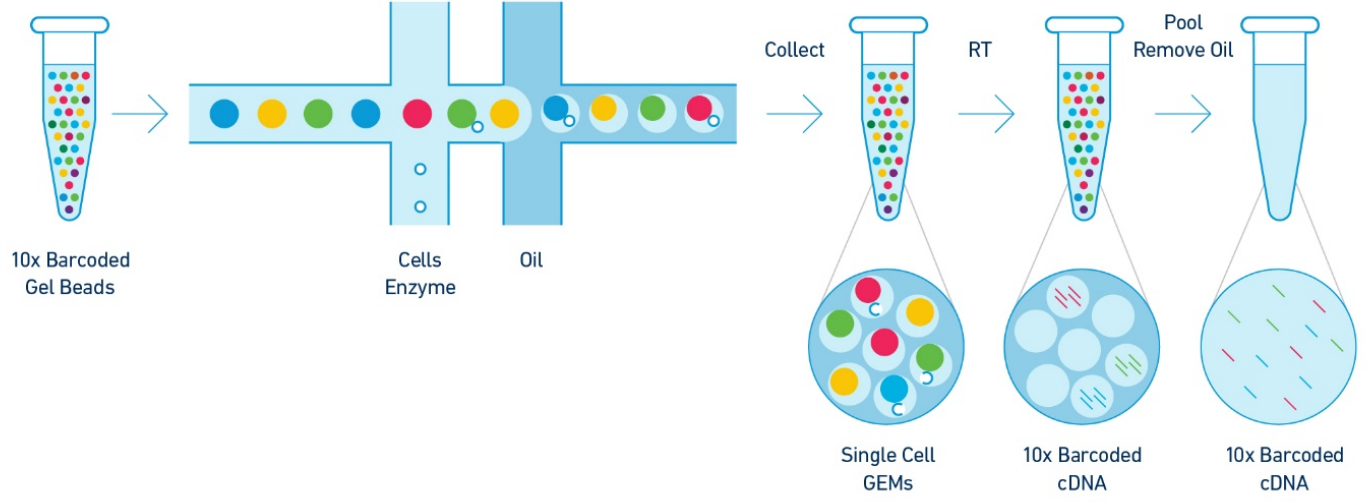
\includegraphics[width=.9\textwidth]{figures/10x_pipeline.png}
    \caption{Описание технологии 10x genomics VDJ: На вход поступает клеточная суспензия определенной плотности. Клетки вместе с реагентами реакции проходят через микрофлюидный (микрогидродинамический) канал, смешиваются с гелевыми шариками и лизисным буфером из другого канала и формируют капли, изолированные друг от друга маслом. На поверхности гелевых шариков находятся баркодированные олигонуклеотиды. Внутри капли за секунды происходит лизис клетки, и содержимое клетки, в том числе молекулы матричной РНК, оказывается внутри капли. Молекулы мРНК гибридизуются с олигонуклеотидами на поверхности шариков, и затем внутри капли происходит обратная транскрипция молекул мРНК в молекулы кДНК. Затем капли <<лопаются>>, полученная библиотека кДНК амплифицируется с помощью ПЦР и отправляется на секвенирование}
    \label{10x_pipeline}
\end{figure}

\begin{figure}[h!]
    \centering
    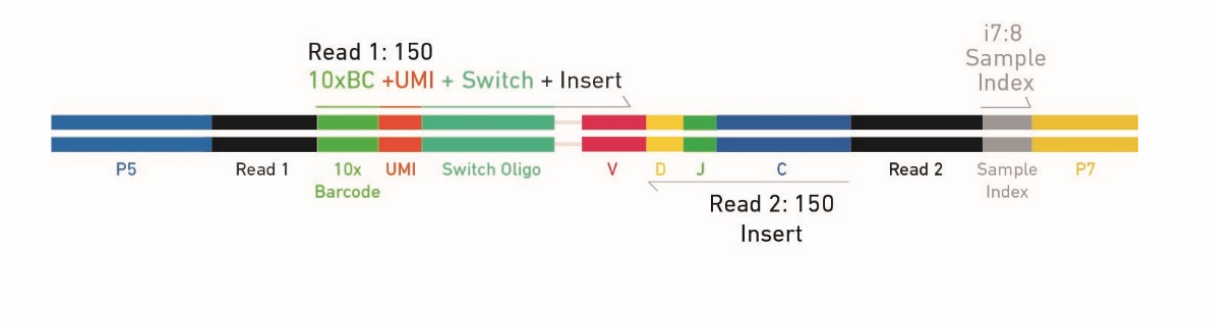
\includegraphics[width=.9\textwidth]{figures/10x_barcodes.png}
    \caption{Структура библиотеки: левый рид покрывает клеточный (16 нуклеотидов) и молекулярный (10 нуклеотидов) баркод. Оба рида являются стандартными парными ридами для технологии Illumina и используются для того, чтобы покрыть вставку.}
    \label{10x_barcodes}
\end{figure}

% Сколько цепей может экспрессировать В-клетка
Известно, что при созревании В-лимфоцитов происходит аллельное исключение, то есть успешная VDJ-рекомбинация гена, который кодирует тяжёлую цепь иммуноглобулина на одной хромосоме, блокирует  рекомбинацию в гомологичной хромосоме. Однако существует исследование~\cite{barreto2000frequency}, в котором было показано, что у здоровых мышей в $1$ случае из $10000$ может происходить одновременная экспрессия обеих тяжелых цепей в IgM+ В-клетках селезенки. Авторы статьи предложили несколько моделей, которые могли бы объяснить данное явление, но пока эти гипотезы не подтверждены. У человека неизветны случаи, в которых В-клетки экспрессируют несолько тяжелых цепей, но есть исследование, в котором было показано, что $30\%$ клеток гибридомы (гибридная клеточная линия, которая получена в результате слияния B-лимфоцитов, полученных из селезёнки иммунизированного животного и опухолевых клеток миеломы) имели дополнительные тяжелые и легкие цепи. Причем  $1.1\%$ клеток имели дополнительную легкую цепь, а $2.2\%$ --- дополнительную тяжелую и легкую цепь. На текущий момент проведено множество исследований (~\cite{pelanda2014dual}, ~\cite{casellas2007igkappa}, ~\cite{liu2005receptor}, ~\cite{fraser2015immunoglobulin}), которые подтверждают, что В-клетки могут экспрессировать две легкие цепи как одного, так и разных типов. Большинство таких В-клеток экспрессируют две легкие каппа-цепи, но редко могут экспрессировать две лямбда-цепи и цепи разных типов. Обычно одно экспрессируемое антитело получается аутореактивное, а второе нормальное, которое позволяет В-клетке обмануть негативную селекцию, созреть, активироваться и дифференцироваться. Считается, что В-клетки  с несолькими легкими цепями встречаются в ???? (малом, меньше $1\%$) случаях.     

% Что мы ожидаем от данных
Таким образом, мы ожидаем увидеть в парных данных, что большинство В-клеток экспрессируют одну легкую и одну тяжелую цепь и редко одну тяжелую и две легких цепи. При секвенировании мы можем увидеть не все цепи, так как они могли не проэкспрессироваться на момент эксперимента. Поэтому мы также ожидаем увидеть в данных клетки, которые имеют только легкую или только тяжелую цепь. Клетки, у которых просеквенирован нестандартный набор цепей, например несколько тяжелых и больше двух легких цепей, скорее всего являются артефактом секвенирования и получились в результате коллизии, при которой больше одной клетки попадали в каплю с молекулярными баркодами. 10х genomics утверждают~\cite{10x_manual}, что вероятность коллизии зависит от концентрации клеток в семпле, и варьируется от $0.4\%$ до $7.6\%$.

% Описание датасетов
Для того, чтобы изучить специфику парных данных 10x, были проанализированы публичные В-клеточные датасеты~\cite{10x_datasets}: 
\begin{enumerate}
    \item CD19 --- B-клетки с маркером CD19, которые были выделены из мононуклеарных клеток периферической крови здоровых доноров. Так как этот вид клеток экспрессирует небольшое количество РНК, библиотека прошла целевое обогащение;
    \item GM12878 --- В-лимфобластоидная клеточная линия с высоким уровнем транскрипции иммуноглобулинов;
    \item NSCLC --- целевое обогащение иммуноглобулинов B-клеток, которые были получены во время свежего хирургического удаления немелкоклеточного рака легкого.
\end{enumerate}

Помимо стандартных типов цепей иммуноглобулинов --- тяжелая, легкая каппа и легкая лямбда, аннотируют последовательности еще одним типом --- мультицепь. Мультицепь --- это последовательность, которая выравнивается на гены разных типов, например V ген выравнивается на каппу-цепь, а J ген на лямбду. На практике оказалось, что в мультицепи попадают последовательности, которые были неправильно проаннотированы. Например, последовательность TGACGGCAGTGAACGC\-1\_contig\_4 из датасета CD19 (подтверждена $83$ молекулярными баркодами) в аннотации 10х имеет IGLV3-21 и IGHJ6 гены, хотя IgBLAST проаннотировал этот контиг генами IGLV3-21*02 и IGLJ1*01 с хорошим качеством выравнивания. Также в аннотациях 10х встречаются последовательности, которые содержат одновременно T и В-клеточные гены, но на самом деле они содержат лишь какие-то подпоследовательности генов иммуноглобулинов (рис.~\ref{IgBLAST_multi}). Мы предполагаем, что в парные данные также попадает РНК, которая транскрибируется из иммунного локуса, и 10х не отфильтровывает такие контиги, а пытается проаннотировать. 

\begin{figure}[h!]
  \centering
  \begin{subfigure}{\linewidth}
    \centering
    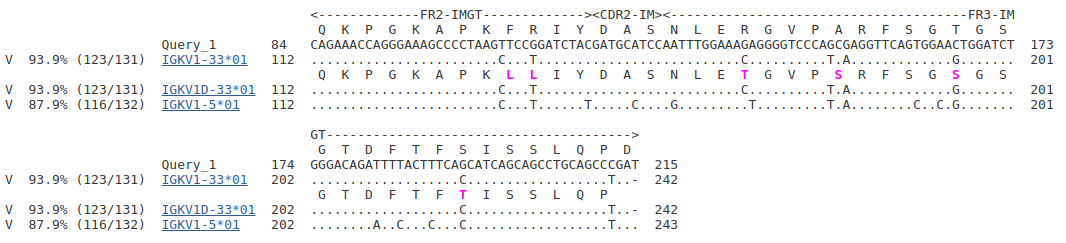
\includegraphics[width=1\textwidth]{figures/IgBLAST_bcr.png}
    \caption{Аннотация контига IgBlAST с выравниванием на базу В-клеточных генов иммуноглобулинов}
  \end{subfigure}

  \begin{subfigure}{\linewidth}
    \centering
    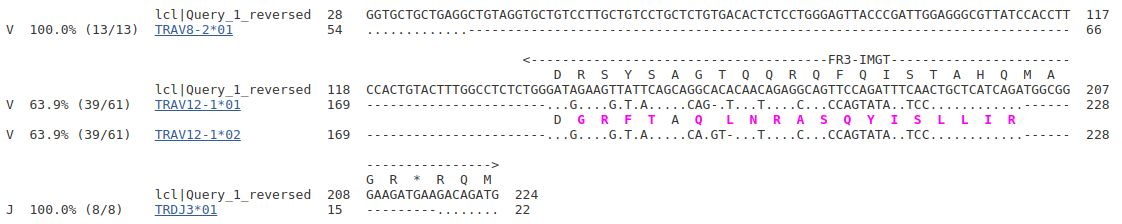
\includegraphics[width=1\textwidth]{figures/IgBLAST_tcr.png}
    \caption{Аннотация контига IgBlAST с выравниванием на базу Т-клеточных генов иммуноглобулинов}
  \end{subfigure}  
  \caption{Пример последовательности, которая проаннотирована 10х как мультицепь с Т-клеточным геном TRAJ22  и В-клеточными геном IGKV2D-28 (контиг GAACATCTCGGCGGTT\-1\_contig\_4 из датасета CD19, подтвержден $65$ баркодами). Из аннотации IgBLAST видно, что последовательность плохо выравнивается на обе базы генов, а также в ней не содержатся гены, которые были указаны 10х.} 
  \label{IgBLAST_multi}
\end{figure}  

Во всех датасетах мы дополнительно отфильтровали контиги, которые подтверждены небольшим количеством молекулярных баркодов (меньше $10$), потому что такие контиги с большой вероятностью являются шумом, например, это могут быть контиги внеклеточной РНК.

Для того, чтобы проверить точность аннотации данных с помощью 10х, мы сравнили ее с IgBLAST, который считается золотым стандартом аннотации иммуных последовательностей. Результат сравнения приведен в таблице~\ref{10x_vs_IgBLAST}. Из таблицы видно, что ДОПИСАТЬ.

\begin{table}[h!]
\centering
\begin{tabular}{|l|l|l|l|}
\hline
                    & \textbf{CD19} & \textbf{GM12878} & \textbf{NSCLC} \\ \hline
\# клеток в датасете                           &      &         &       \\ \hline
\# всех цепей в датасете                       &      &         &       \\ \hline
\% цепей отфильтрованных IgBLAST               &      &         &       \\ \hline
\% мультицепей                                 &      &         &       \\ \hline
\% мультицепей, которые проаннотировал IgBLAST &      &         &       \\ \hline
\% цепей с совпавшими аннотациями V генов      &      &         &       \\ \hline
\% цепей с совпавшими аннотациями J генов      &      &         &       \\ \hline
\% цепей с совпавшими аннотациями V и J генов  &      &         &       \\ \hline
\end{tabular}
\caption{Сравнение 10х аннотатора и IgBLAST}
\label{10x_vs_IgBLAST}
\end{table}

% Статы по количеству цепей в клетке
Из таблицы~\ref{stats_nchains} видно, что существенный процент клеток имеет $3$ цепи, что противоречит нашим ожиданиям. Для того, чтобы подтвердить, что это действительно разные цепи, а не артефакты технологии секвенирования и ПЦР, мы построили гистограмму расстояний между двумя цепями одного типа, которые находятся в одной клетке. Из графиков~\ref{chains_hist} видно, что цепи делятся на два кластера разного размера, но при этом цепи в большем кластере сильно различаются. Таким образом, в парных данных 10х большее число клеток с тремя цепями, чем ожидалось из предыдущих исследований. 

\begin{table}[h!]
\centering
\begin{tabular}{|l|l|l|l|l|l|l|l|}
\hline
        & \textbf{1 цепь} & \textbf{2 цепи} & \textbf{3 цепи} & \textbf{4 цепи} & \textbf{5 цепей} & \textbf{6 цепей} & \textbf{\textgreater{}6 цепей} \\ \hline
CD19    & 22.67\%         & 63.26\%         & 10.53\%         & 2.7\%           & 0.69\%           & 0.14\%           & 0.01\%                         \\ \hline
GM12878 & 17.51\%         & 56.80\%         & 21.66\%         & 4.03\%          & 0.00\%           & 0.00\%           & 0.00\%                         \\ \hline
NSCLC   & 51.26\%         & 46.55\%         & 2.02\%          & 0.17\%          & 0.00\%           & 0.00\%           & 0.00\%                         \\ \hline
\end{tabular}
\caption{Процентное соотношение клеток по количеству экспрессируемых цепей}
\label{stats_nchains}
\end{table}

 
 \begin{figure}[h!]
    \centering
    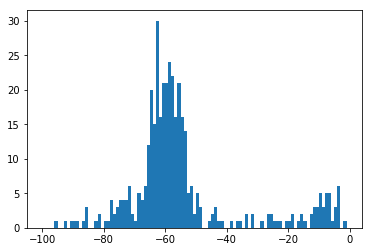
\includegraphics[width=.9\textwidth]{figures/HKK_hist.png}
    \caption{ПЕРЕРИСОВАТЬ НОРМАЛЬНО И ДЛЯ ВСЕХ (конкретно этот случай для 1 тяжелой и 2 каппы). Распределение расстояния между кратными цепями в клетках, которые содержат $3$ цепи.  В качестве расстояния между двумя цепями было взято расстояние редактирования со следующими штрафами: $0$ за совпадение, $-1$ за несовпадение, $-0.5$ за открытие гэпа и $-0.1$ за его продолжение.}
    \label{chains_hist}
\end{figure}

   

% Статы по типам клеток








% -------------------------------------------------------------------------------------------

\section{Симулятор парных данных}

Так как реальные данные странноваты, мы будем моделировать (непонятно, как ведут себя несколько легких цепей с точки зрения дерева. Отбор идет только по одной или обеим?). Частоты цепей возьмем из статьи~\cite{dekosky2015depth}. 


% -------------------------------------------------------------------------------------------

\section{Описание алгоритма}

В процессе осмысления



% У заключения нет номера главы
\section*{Заключение}

\bibliographystyle{ugost2008ls}
\bibliography{diploma.bib}
\end{document}
